\chapter{Metodologia}
  \section{Gerenciamento}
    \subsection{Estrutura Analítica do Projeto (EAP)}

      Tendo como objetivo a visão geral sobre as atividades que serão
      realizadas no decorrer do projeto, escolheu-se a EAP como forma
      de organização sistematizada das informações.

      A EAP consiste em uma organização das entregas
      a serem feitas em um formato de árvore, partindo de tarefas
      mais gerais para tarefas mais específicas \cite{pmbok2012}.

      Para a construção da EAP, foram levados em conta as diferentes
      entregas a serem realizadas dentro do ciclo de vida do projeto,
      assim como as áreas de atuação dentro da equipe. Além disso, é
      possível observar o alinhamento da EAP com as atividades previstas
      no cronograma e com os requisitos estabelecidos para o projeto.

      A figura \ref{fig:eap} é a representação gráfica da EAP do projeto.

      \begin{figure}[!htbp]
        \centering
        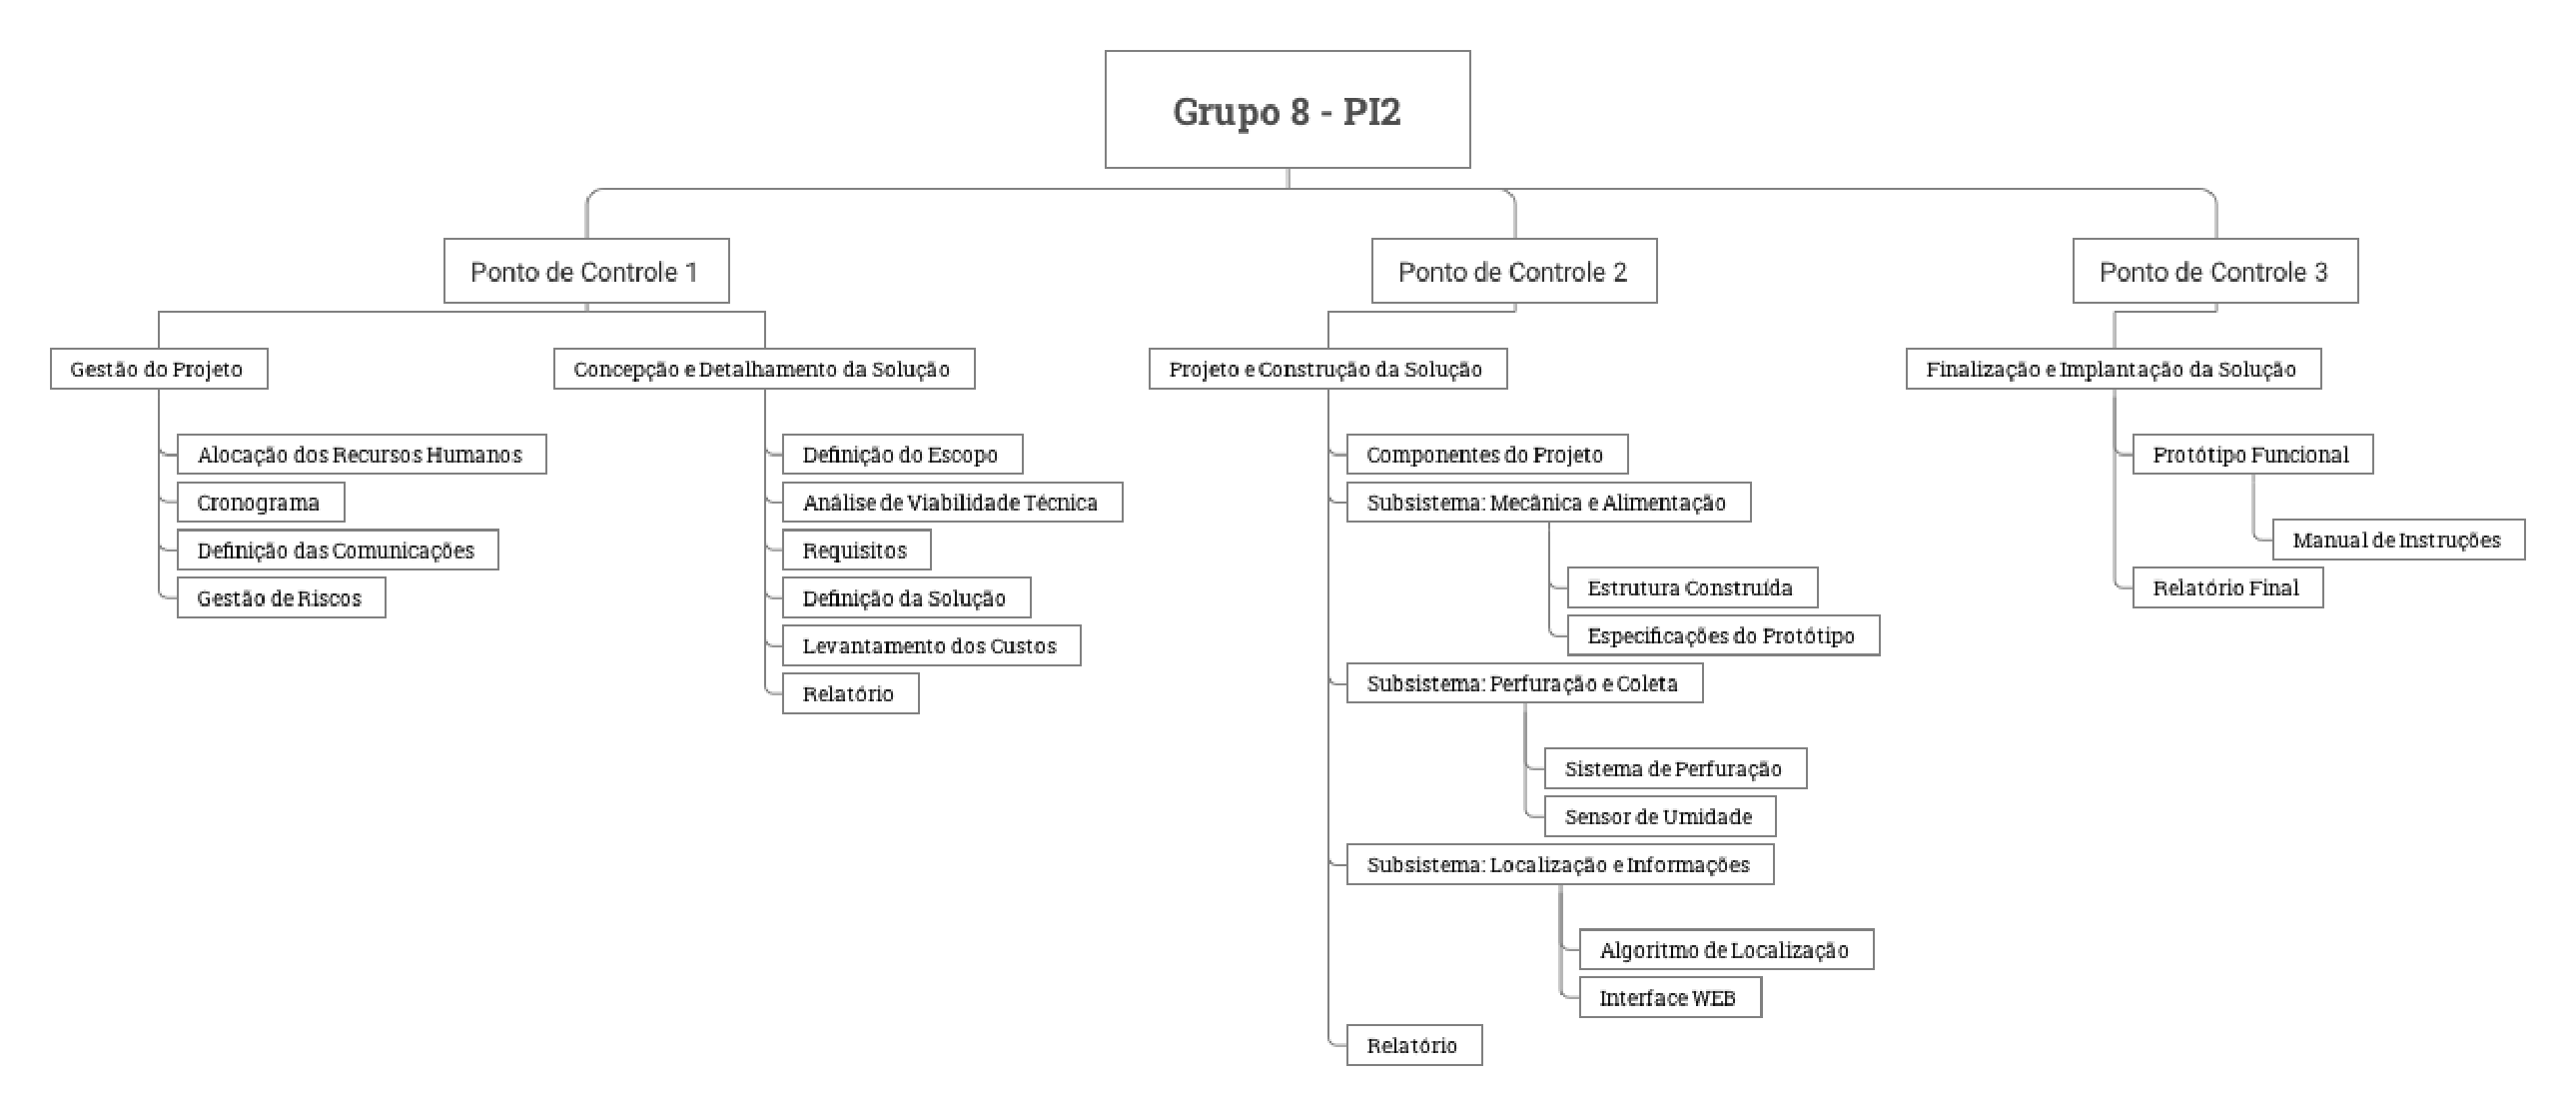
\includegraphics[width=\textwidth]{figuras/EAP.eps}
        \caption{Estrutura Analítica do Projeto. Fonte: autores.}
        \label{fig:eap}
      \end{figure}

      \vfill
      \pagebreak

    \subsection{Alocação dos Recursos Humanos}
	Para este projeto foram designados treze alunos de cinco cursos de engenharia da Universidade de Brasília. Os alunos foram escolhidos dos cursos de Engenharia Aeroespacial, Engenharia Automotiva, Engenharia Eletrônica, Engenharia de Energia e Engenharia de Softwre. Com base nas engenharias foi dividido o trabalho em quatro frentes de atuação sendo elas:
	\begin{itemize}
		\item \textbf{Software}: responsável pela implementação do aplicativo e comunicação com os microcontroladores.
		\item \textbf{Eletroeletrônica}: responsável pela implementação dos microcontroladores e acionamento do motor.
		\item \textbf{Alimentação}: responsável por todo suprimento energético.
		\item \textbf{Estrutura}: responsável por desenhar e elaborar a estrutura do veículo.
	\end{itemize}
	
	A figura \ref{img:projeto} apresenta as áreas de trabalho com os seus integrantes. Os integrantes foram alocados de acordo com a especialidade e conhecimento adquirido durante o curso de graduação.
	
	\graphicspath{{figuras/}}
	\begin{figure}[h!]
	\centering
	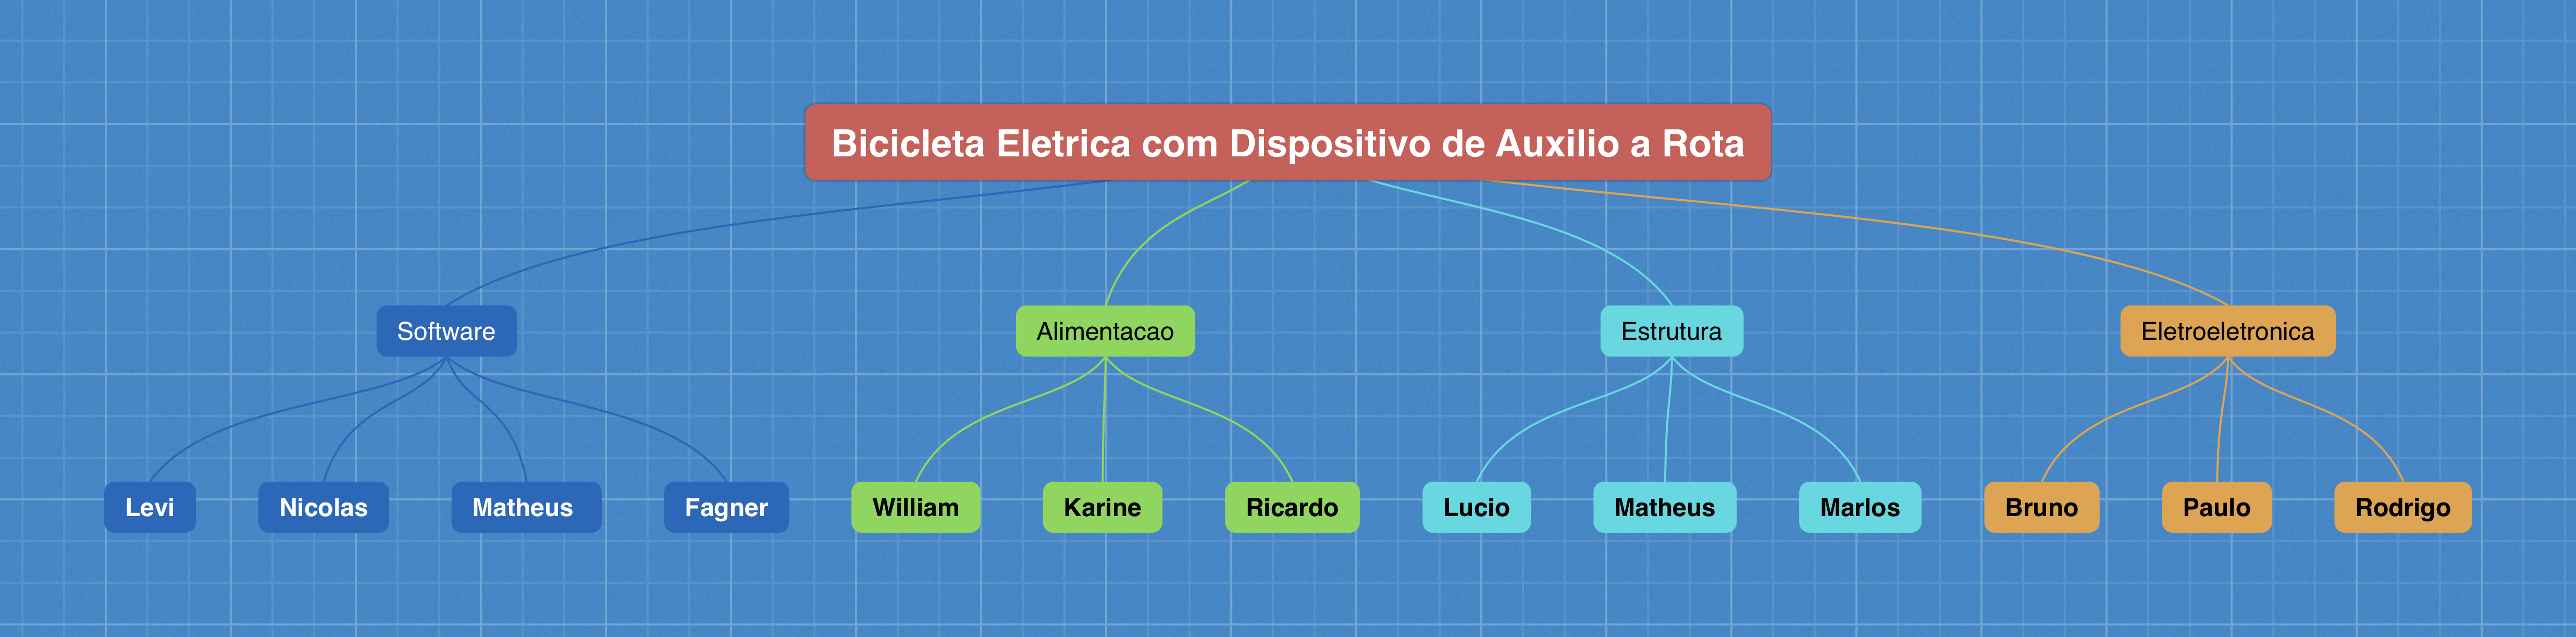
\includegraphics[scale=0.20]{project.png}
	\caption{Áreas de desenvolvimento e seus respectivos integrantes}
	\label{img:projeto}
	\end{figure}


    \subsection{Comunicação}

      Para que qualquer projeto tenha sucesso é necessário o engajamento da equipe, sendo assim, é necessário uma comunicação eficaz entre os membros da equipe. A tabela \ref{tab:com} detalha os métodos de comunicação utilizados pela equipe.
      
      \begin{table}[!htbp]
      	\begin{center}
      		\caption{\label{tab:com}Métodos de comunicação. Fonte: autores.}
      		\begin{tabular}{|p{4cm}|p{4cm}|p{3cm}|p{3cm}|p{2cm}|}
      			\hline
      			\textbf{Objetivos} & \textbf{Ferramenta} & \textbf{Frequência} & \textbf{Horário} & \textbf{Local}\\\hline\hline
      			Acompanhamento das atividades & Kanban & Sob demanda & Horário da disciplina & FGA\\\hline
      			Avisos rápidos / Lembretes & Telegram & Sob demanda & N/A & N/A\\\hline
      			Decisões Técnicas/Planejamentos & Presencial & Duas vezes por semana & Horário da disciplina & FGA\\\hline
      			Desenvolvimento do projeto & Google Docs/ Google Hangouts/ Git / Github / Presencial & Sob demanda & Durante desenvolvimento do projeto & N/A\\\hline
      		\end{tabular}
      	\end{center}
      \end{table}

    \subsection{Tempo}
	O cronograma serve como uma ferramenta de gerenciamento do tempo, onde são colocados datas de início e término das atividades. Neste tópico é apresentado uma versão completa de como foi organizado o cronograma para gerenciamento do tempo do grupo. Um cronograma contendo o detalhamento das atividades é apresentado no apendice deste documento.

	Como é possível ver na figura \ref{img:cronograma_geral}, o projeto foi dividido em 3 grandes marcos (Pontos de Controle). As atividades se alinharam de acordo com o que é esperado em cada marco. No primeiro marco, as entregas são focadas na definição das tecnologias e na forma como será elaborado o produto final. O segundo marco tem como objetivo, a implementação do produto específico de cada área de conhecimento (Alimentação, Software, Estrutura e Eletroeletrônica). Ao fim do terceiro e último marco, espera-se que todas as áreas sejam capazes de integrar o produto desenvolvido no marco 2. 

	\graphicspath{{figuras/}}
	\begin{figure}[h!]
	\centering
	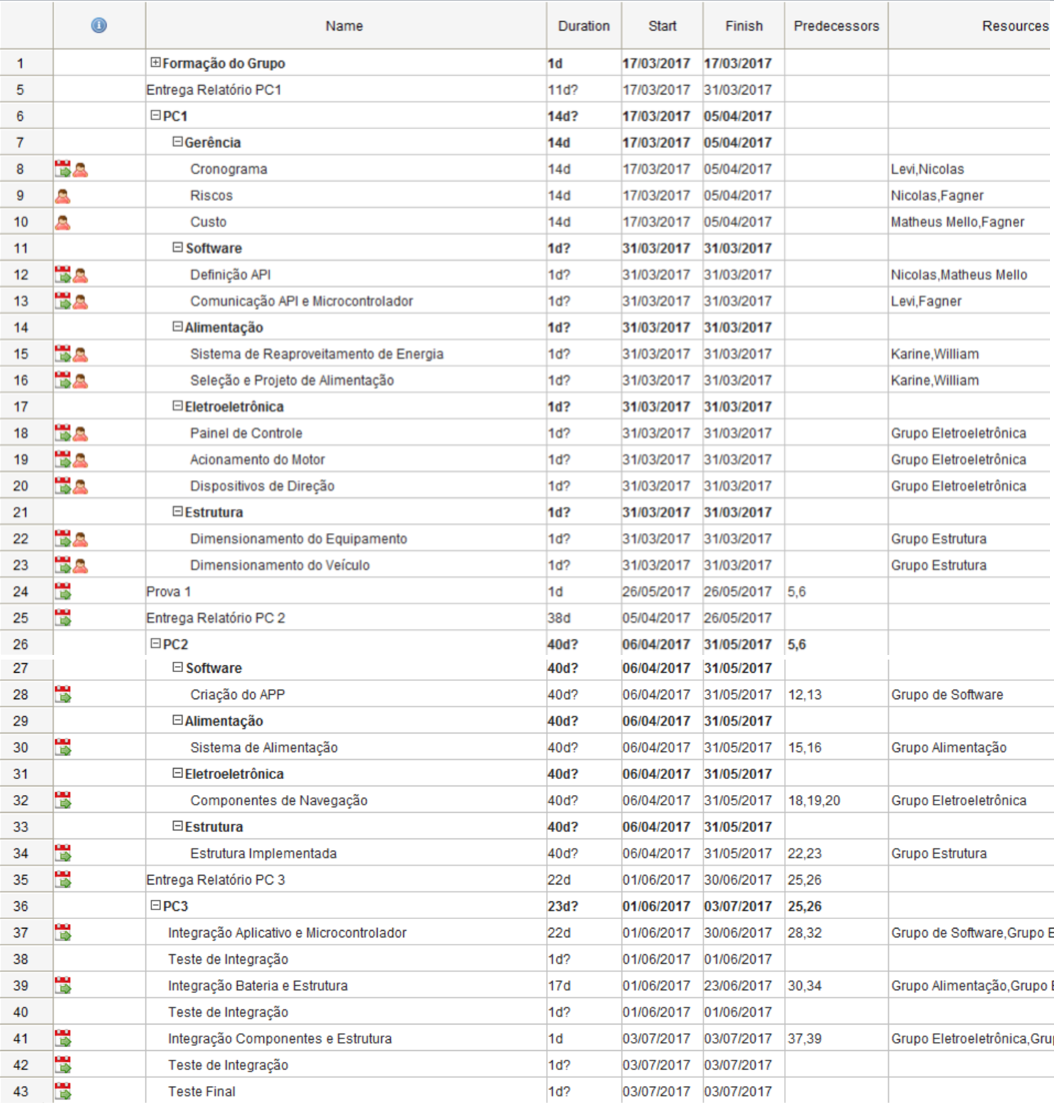
\includegraphics[scale=0.80]{cronograma_geral}
	\caption{Cronograma geral do projeto}
	\label{img:cronograma_geral}
	\end{figure}